% !TEX root = main.tex
\subsubsection {Spontaneous association with cholesterol in binary membranes} \label{binary}

For the purpose of this article nAChR is colored: $\alpha$:green, $\gamma$:cyan, $\delta$:gray, $\beta$:purple. C16:0 is blue, DHA is white, LA is tan, and Chol is red.

In simulations of a single nAChR in systems containing DPPC and 0-40\% cholesterol, measurements (trajectories shown in Fig \ref{fig:binary}A) of $Q_{DPPC}$ indicated moderate depletion of DPPC among nAChR boundary lipids (Figure \ref{fig:binary}B lower).  Two-dimensional heat maps of the local cholesterol density reveal that at low concentrations of cholesterol, this depletion is almost entirely within ``embedded'' or non-annular lipids that are at least partially buried within the protein bundle (Figure \ref{fig:binary}C) as predicted in \cite{Brannigan_Embedded_2008}.

Saturation of such non-annular sites is apparent in the plateau in $Q_{DPPC}$ between 10 and 20\% cholesterol, which is remarkably consistent with the concentration of cholesterol typically required in reconstitution mixtures to restore native function.  \cite{reconstitute}  Intriguingly, all simulations consistently yielded four general regions of differential embedded cholesterol density : a high density region ($\alpha-/\gamma+$ interface and center of the $\alpha$ subunit), a low/background density region ($\alpha-/\beta+$ interface and center of $\beta$ subunit) on the opposite face of the TMD, and two regions of intermediate density that separated them.  In the absence of nAChR, DPPC/CHOL lipid bilayers are randomly mixed, and this result indicates an intrinsic cholesterol ``amphipathic''.  

At higher concentrations of cholesterol, cholesterol was also enriched in ``annular'' sites, particularly at the high affinity and low affinity face of the TMD.  This enrichment actually extended many lipidation shells off the high affinity face, indicating nAChR was not just sorting lipids, but even inducing organization of the membrane. Enrichment far from the TMD is expected to be particularly sensitive to finite size effects, although there is no clear reason for why these effects would consistently have a dependence on protein orientation.  
% , and two intermediate density regions (1: $\gamma-/\alpha+$ face and subunit center of both subunits and 2: ) and $\delta-/\alpha+$ faces, and nearly background density on the $\alpha-/\beta+$ face.  As a result, the protein overall 

\begin{figure*}[h!]
	\center
	\includegraphics[width=1\linewidth]{DPPC_Only.pdf}
	\caption{Analysis of binary systems comprised of DPPC and cholesterol A: Trajectory of nAChR in DPPC:CHOL 80:20 over various time steps. System starts randomly mixed, by 2$\mu s$ boundary lipids are moderately deleted of DPPC. B: $M_{DPPC}$ and $Q_{DPPC}$ shown over various concentrations of cholesterol. C: Density plots 50 \AA from origin. Showing DPPC (left) and CHOL (right) using radial coordinates.}
	\label{fig:binary}
\end{figure*} 

\subsubsection {Domain formation in lipid bilayers containing PUFAs} \label{Demix}

	Addition of phospholipids with unsaturated acyl chains to systems containing a saturated lipid and cholesterol is well-established to induce domain formation, and polyunsaturated phospholipids make these domains more well-defined\cite{levitalraft} and can even sometimes induce domain formation in binary membranes.\cite{weirdpaper} In these simulations, non-random mixing (including domain formation) was measured via $M_{a,b}$.  Enrichment of lipid species $b$ among the nearest neighbors of lipid species $a$ is quantified by $M_{a,b}$ (see equation \ref{eq:M}), with values close to 0 indicating random mixing, and positive and negative values indicating enrichment or depletion of species $b$ around species $a$, respectively.  Positive values of $M_{a,a}$ close to 1 indicate substantial demixing.  
	
	Addition of PUFAs to DPPC/CHOL bilayers in the absence of nAChRs did induce phase separation, as indicated by the symbols in Figure \ref{fig:fig2}.  Adding a single nAChR did not change values for $M$; i.e. the observed domains resulted from the lipid composition and were not dependent upon the presence of the protein.  Across systems (Figure \ref{fig:fig2} \textbf{a}), maximum values of $M_{DHA,DHA}$ approached 5, and were significantly reduced (to less than 0.5) when DHA chains were replaced with LA chains. This result is consistent with that of \cite{Levental_Polyunsaturated_2016} where a significant increase in miscibility temperature was observed upon supplementation of plasma membranes with $n-3$ lipids.  
	
	  %and  while  increases as the molar fraction of DHA-PE is reduced from the membrane, implying increased enrichment at reduced concentrations. 
	As shown in Figure \ref{fig:fig2}\textbf{a},  $M_{DHA,DHA}$ actually increases as the molar fraction of DHA-PE is reduced from the membrane, implying increased self-association of DHA at reduced concentrations of DHA, with even the lowest concentrations of DHA that we used here seemingly higher than the critical miscibility concentration.  $M_{DHA,DHA}$ is not sensitive to the ratio of cholesterol vs saturated lipid, at least over the compositions simulated.   Relative to systems containing DHA, $M_{LA,LA}$ is miscible, with small amounts of domain formation sensitive to the CHOL:DPPC ratio; an apparent maximum for $M_{LA,LA}$ occurs near 20\% LA, 20\% Cholesterol, and 60\% DPPC.  

	\begin{figure*}[t]
		\center
		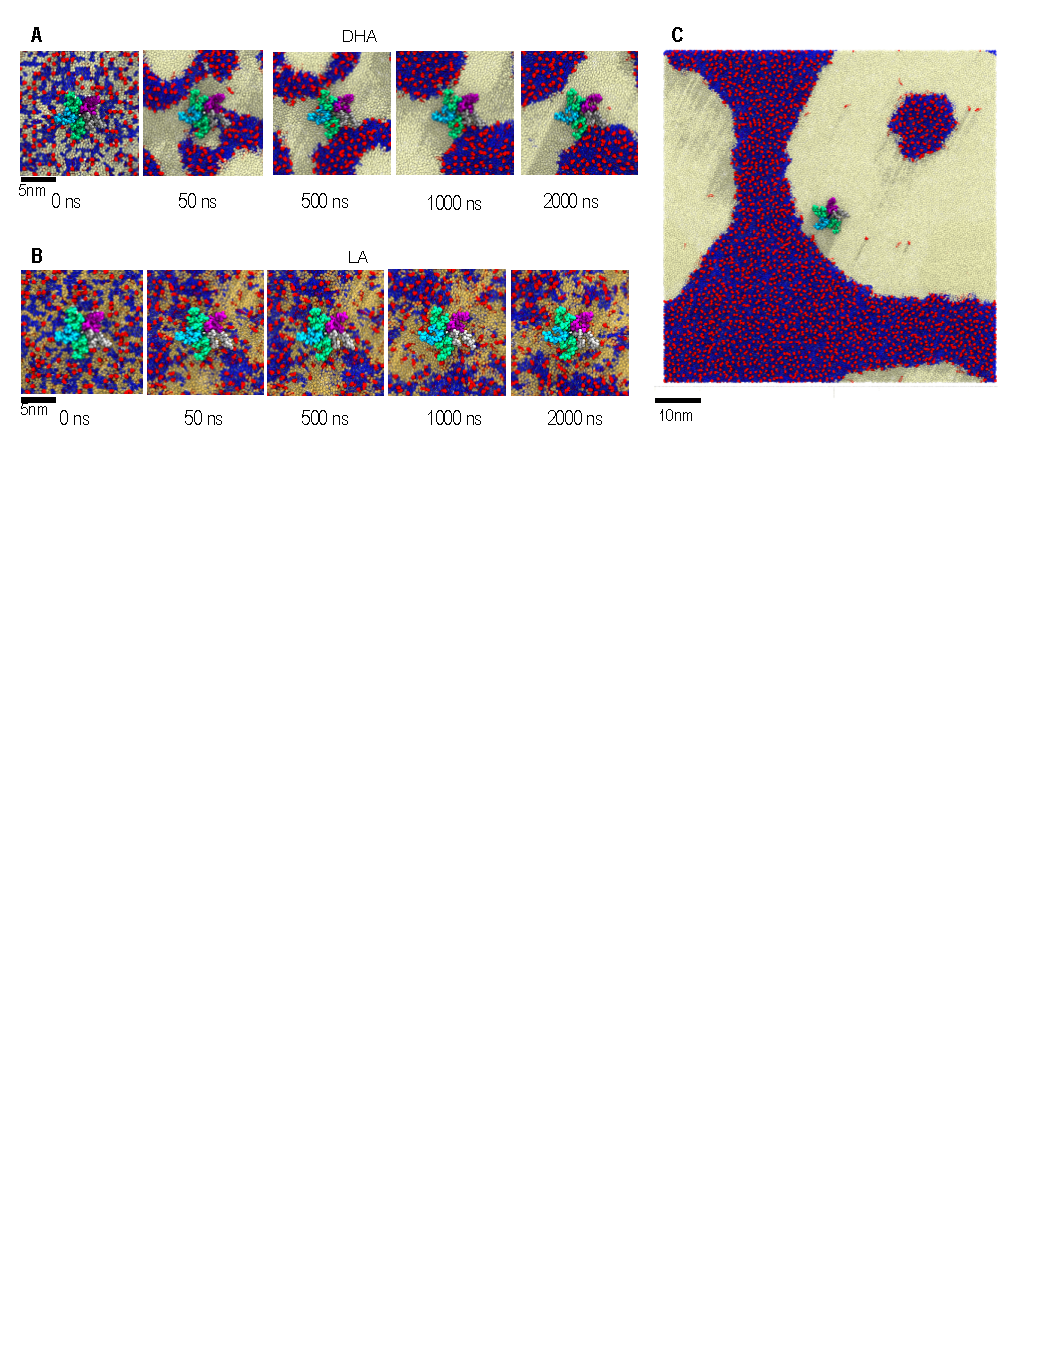
\includegraphics[width=1\linewidth]{Fig1.pdf}
		\caption{ A,B: Figure show de-mixing trajectories of various lipid compositions.  A: Trajectory shows a systems of DHA-PE, DPPC, and Chol (40:40:20) de-mixing with nAChR exploring the membrane. B: Trajectory shows a systems of DLiPC, DPPC, and Chol (40:40:20) de-mixing with nAChR exploring the membrane. C: Image shows system with membrane of $75x75$ $nm^2$.} 
		\label{fig:fig1}
	\end{figure*}
%	Removing nAChR from the simulation system does not significantly alter domain formation or measured values of $M_{LA,LA}$ or $M_{DHA,DHA}$,   The value of the differences in $M_{a,b}$ between membrane only and membrane with protein systems are provided in SI \ref{fig:diff}. 
	%indicating the most cohesive domains, were observed for amounts of $x_{Chol}$ < 20\% and DPPC < 40\%. Figure \ref{fig:fig2} \textbf{a right} shows $M_{LA,LA}$ is greatest when DLiPC is at molar fraction of $\sim 30$\%. Increasing a simulations box size, or increasing the number of proteins, has not appeared to alter these results. The concentration space of DHA and LA shows DHA's ability to form domains is dependent on $x_{DHA}$ and $x_{Sat}$, while DLiPC domains tend to be approximately consistent. 
%	nAChR does not prevent domain formation, it does shift de-mixing values. In simulations lacking proteins, but containing PUFAs, membranes separate into two phases. 

	%Figure \ref{fig:fig2} \textbf{a} shows lipid-lipid interaction; the contour surface represents systems including a protein, and the symbols represent systems lacking a protein. 
	
	Similarly as shown in Figure \ref{fig:SIQ} %\ref{fig:OL}, 
	these results were insensitive to headgroup (PE or PC) for the compositions simulated.  %shows three other systems of X:DPPC:Chol, where X is DHA-PC, DLiPE, and DPPE. The lipids containing PUFAs (DHA-PC and DLiPE) shared similar traits to DHA-PE and DLiPC. DPPE appeared to mix $\sim$ randomly with DPPC and Chol.
	%GB: let's talk about the above
	This is consistent with previous work \cite{Inglfsson_Lipid_2014,Risselada_The_2008,Perlmutter_Interleaflet_2011,Veatch_Organization_2002} indicating domain formation in ternary mixtures to be primarily dependent on differences in acyl chain unsaturation and relatively insensitive to head group.   %in ternary mixtures using unsaturated and saturated lipids with cholesterol form $l_o$ and $l_d$ domains, without sensitivity to head groups.

%	The difference in $M_{a,b}$ ($\Delta M_{a,b}$) between membrane only and membrane with protein systems are shown in SI \ref{fig:diff}. %Systems with LA $\Delta M_{a,b}$ values remain within $\sim 0.0\pm 0.3$. Comparatively, systems with DHA show divergence from the expected 0.0 as the concentration of DHA decreases, similar to Figure \ref{fig:fig2}a.
	The well-defined boundaries between domains that were found in systems containing DHA-PE are also observed in systems containing DHA-PC. Shorter acyl chains and greater saturation did not promote well defined domains as seen using DHA (see Figure \ref{fig:fig1}A). DHA is a relatively long chained n-3 fatty acid making it highly flexible. DHA has been shown to stabilize $l_{do}$ domain formation \cite{Levental_Polyunsaturated_2016,Lor2015}.  It may be the case running our simulations for longer time would produce well defined domains for any PUFA \cite{Risselada_The_2008}.

\subsubsection{nAChR Partitioning Preference} \label{PUFA}
	For all lipid compositions tested, nAChR partitioned into the $l_{do}$ phase if one was present, and as shown below, boundary lipids were enriched for unsaturated lipids even in the absence of domain formation.  % within a randomly mixed ternary membrane, then allowing the membrane to de-mix and nAChR to explore domains, reveals nAChR to partition into the $l_d$ domain if a $l_d$ domain is present. 
	This includes all tested concentrations of the ternary mixtures of DPPC, DHA-PE, and Chol (Figure \ref{fig:fig1}A), DPPE, DHA-PC (not shown) ,and Chol, and DPPC, DLiPC, and Chol (Figure \ref{fig:fig1}B).%, albeit not as critically for membranes including DLiPC.
	These results are shown over either zwiterionic head group (PC and/or PE). A comparison of PC and PE head groups with C16:0 and DHA acyl chain preference is shown in Figure \ref{fig:SIQ}. In all four figures nAChR resides in $l_{do}$ phases, reinforcing its dependency on acyl chains.

	%In  heat maps describing the boundary DPPC near nAChR. 
	This result was quantified using a metric notated $Q$ and defined in equation \ref{eq:Q}; negative and positive $Q$ indicate depletion and enrichment DPPC among boundary lipids, respectively.  $Q$ approaching 1 or -1 corresponds to partitioning within a well-defined $\l_{o}$ or $\l_{do}$ phase, respectively. (Figure \ref{fig:fig2}\textbf{b}).%   indicating partitioning within the $\l_{d}$ phase, Q = 0 indicates random partitioning, and Q = 1 indicates enrichment of DPPC lipids, indicating partitioning within the $l_{do}$ phase (Figure \ref{fig:fig2}\textbf{b}).  
	In all systems studied here, $Q < 0$, but in systems containing longer, $n-3$ chains, Q was much closer to -1 than in systems containing shorter, $n-6$ chains.  Selected simulations in which headgroups were swapped suggested this reflected the difference in acyl chain rather than head groups (\ref{fig:fig?}). From $Q$ alone it is not clear whether this difference reflects a significantly higher affinity of nAChR for $n-3$ DHA than $n-6$ LA or simply the more well-defined $l_{do}$ phase formed by DHA compared to LA. 	%The color bar in Figure \ref{fig:fig2}\textbf{b} represents $Q$. 	 
	We did consistently measure $Q<0$ regardless of restraints place on the protein or box size (Figure \ref{fig:fig2} \textbf{c}). % shows harmonic restraints in a membrane $\sim 75x75nm^2$.  

	%fig? was the cth figure in figure one, we replaced it with the large simulation image.

	%Both saturation and acyl chain length dictate domain formation. 
	Trends for $Q$ with changing fractions of unsaturated lipid and cholesterol were highly sensitive to whether $n-3$ or $n-6$ lipids were used.  DPPC has such low affinity relative to $n-3$ lipids for most sites on the nAChR that $B_{DPPC}/N_{B} \le 10\%$ regardless of $x_{DPPC}$. Intermediate amounts of $n-3$ unsaturated lipids (between 30 and 40\%) further depletes DPPC from boundary lipids,  even when  over a wider range of cholesterol ratios.   
	
	%GB GOT TO HERE
	Figure \ref{fig:fig2} \textbf{b} shows boundary lipids are highly dependent on species of PUFA and cholesterol. Figure \ref{fig:fig2}B with DHA demonstrates an approximately constant $Q_{DPPC}$ at cholesterol concentrations between $\sim$0.05\% to $\sim$25\%, maintaining $\sim$ constant DPPC concentration. $Q_{DPPC}$ using the PUFA LA, still has a cholesterol dependence, however LA's affinity to mix with $l_o$ lipids maintains much higher values of $Q_{DPPC}$. $Q$ values appear to be maximum in systems with $\sim$ neuronal and \textit{Torpedo} $x_{Chol}$.

	Results run counter to some experimental interpretations using model membranes \cite{Perillo_Transbilayer_2016,Pato_Role_2008}.
	%Bermdez et al \cite{Bermdez_Partition_2010}, showed nAChR to partitioned equally into $l_o$ and $l_{do}$ domains in model membranes of Chol:POPC:SM 1:1:1. Expanding on \cite{Bermdez_Partition_2010}, Perillo et al \cite{Perillo_Transbilayer_2016} showed using the previous composition but inducing asymmetrical membrane compositions, promoted nAChR to partition into the $l_o$ domain. These results may represent nAChR sitting at an interface instead of in a $l_{do}$ domain (see Section \ref{Interface} and Figure \ref{fig:fig3}). 
	POPC is composed of palmitic (c16:0) and oleic (c18:1) acids with a PC head group. Oleic acid is mono-unsaturated, maintaining a greater order than PUFAs, but less then saturated fatty acids. This combination of acyl chains may create a highly defuse $l_{do}$ phase, increasing the interfacial area, a location where nAChR is frequently observed in these simulations. We observe this is consistent with observations from \cite{Schafer2011}, who showed protein partitioning into the $l_{do}$ phase. %need a source if I want to make that claim...

	\subsubsection{nAChR Preference for Domain Interface Including PUFAs} \label{Interface}

	With the inclusion of PUFAs, our simulations have consistently shown nAChR partitions into the $l_do$ phase. Interestingly, nAChR is recurrently in close or direct contact with the $l_o$ phase, imaged in Figure \ref{fig:fig1}A and C, Figure \ref{fig:SIQ}, Figure \ref{fig:fig3}, and Figure \ref{fig:sum}.

	We predicted that by increasing the membrane area may adjust the nAChR residing at the interface. However, increasing the membrane area to $\sim 75x75$ $nm^2$, nAChR is observed to remain in the $l_{do}$ domains, partitioning near or at the $l_o$-$l_d$ interface, Figure \ref{fig:fig1}C. Using native \textit{Torpedo} electric organ membrane, Unwin 2017 \cite{Unwin_Segregation_2017} supposedly showed nAChR's $\alpha_{-}/\delta_{+}$ subunits found nearby a cholesterol enriched domain. 

	%%PUFAs have been predominantly ignored in nAChR-lipid studies. By including PUFAs, our simulations have consistently shown nAChR partitions into the $l_do$ phase, and in either close or direct contact with the $l_o$ phase, imaged in Figure \ref{fig:fig1}, Figure \ref{fig:fig3}, and Figure \ref{fig:sum}. Increasing the membrane area to $\sim 75x75$ $nm^2$, nAChR is observed to remain in the $l_{do}$ domains, partitioning near or at the $l_o$-$l_d$ interface, Figure \ref{fig:fig1} \textbf{c}. Unwin 2017 \cite{Zuber_Structure_2013} suggested nAChR's $\alpha_{-}/\delta_{+}$ subunits found nearby a cholesterol enriched domain. 

	\begin{figure}[h!]
		\center
		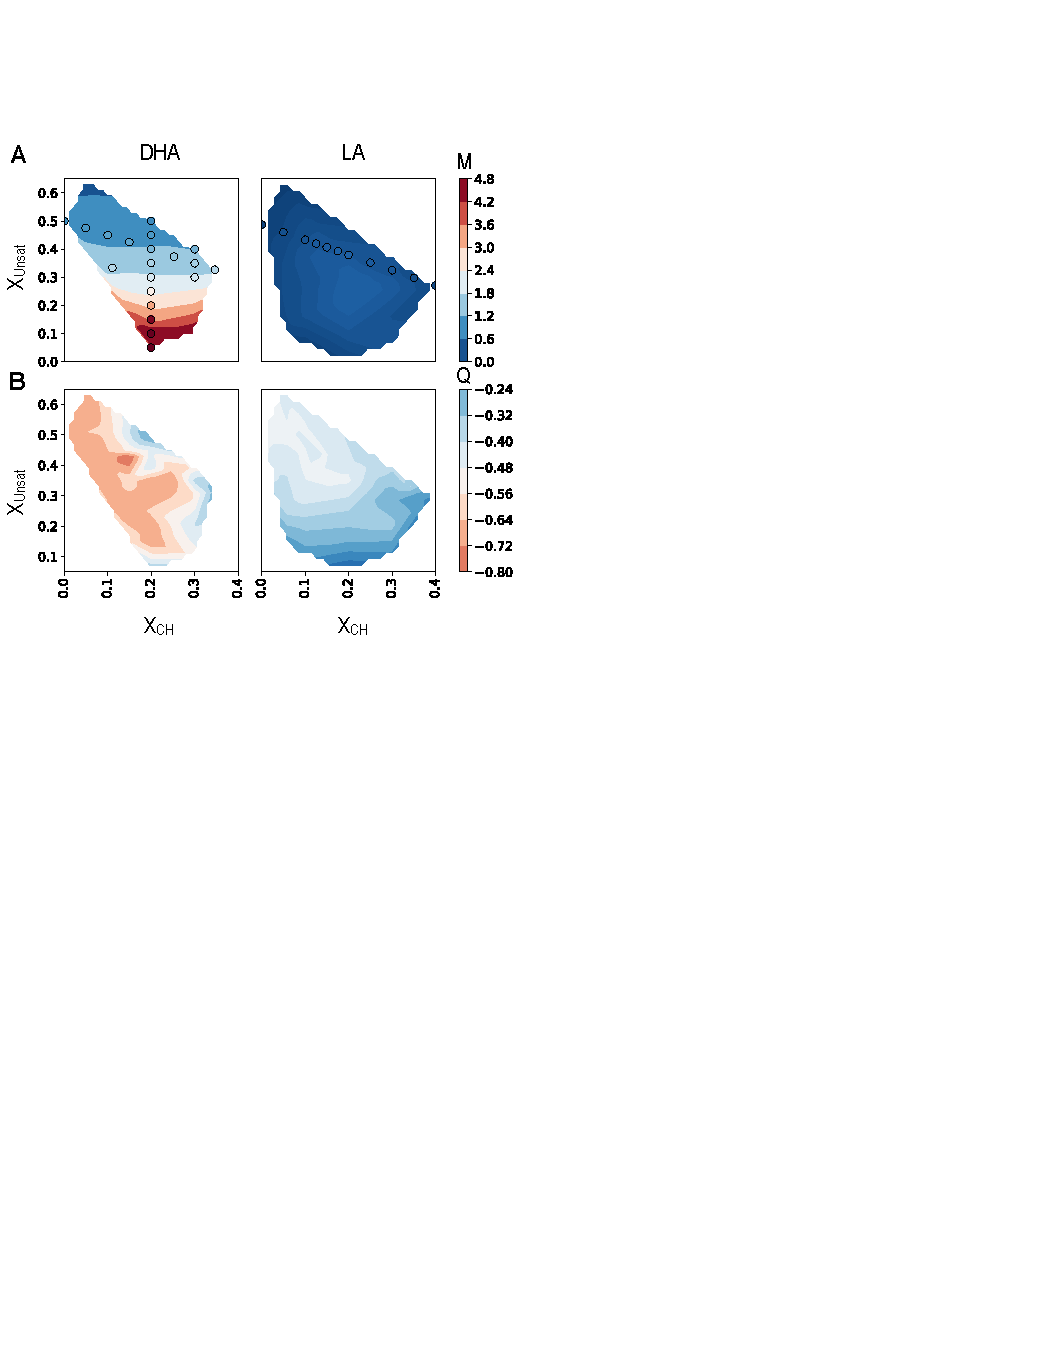
\includegraphics[width=1\linewidth]{Fig2.pdf}
		\caption{A: Plots show $M_{a,b}$ over concentration space of DPPC and Chol. Left: plot Systems with DHA-PE-DHA-PE mixing. Right: plot show DLiPC-DLiPC mixing. B: Plots show $Q$ over concentration space PUFA:Chol. Left: Systems with DHA-PE. Right: Systems with DLiPC.}
		\label{fig:fig2}
	\end{figure} 

	\begin{figure}[!ht]
		\center
		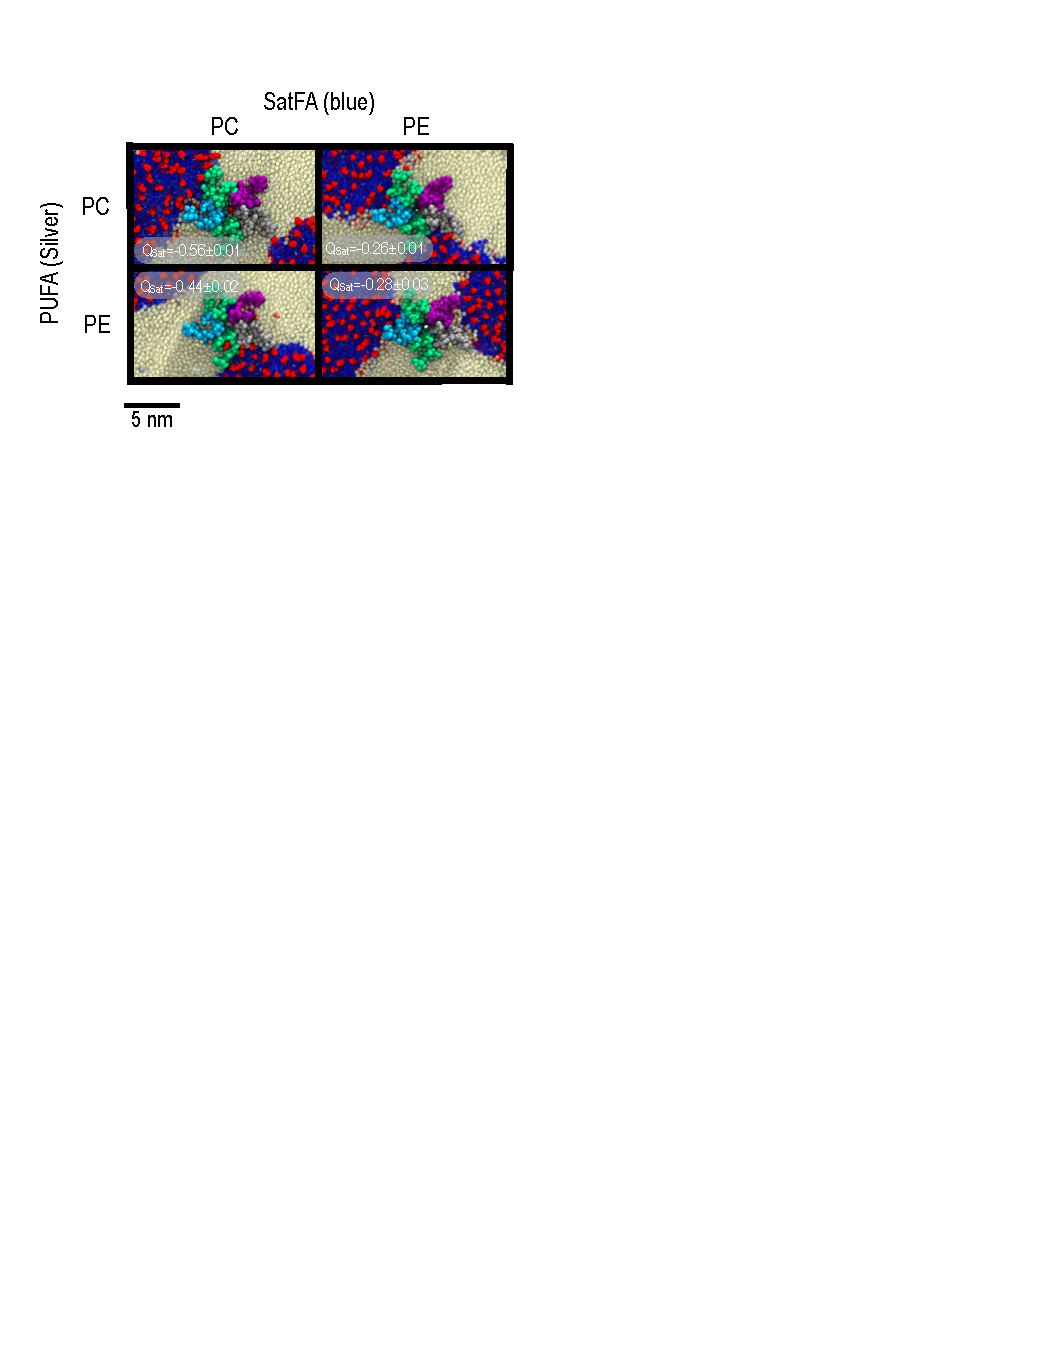
\includegraphics[width=1\linewidth]{SI_Q.pdf}
		\caption{All images are final snap shot of 2$\mu s$ simulations at concentration Sat:PUFA:Cholesterol 40:40:20. Saturated acyl chains are C16:0 and the PUFA is DHA, and head groups are PC or PE.}
		\label{fig:SIQ}
	\end{figure}

	%\subsection{nAChR and Zwitterionic Lipid Head Group Preference} \label{Zwitter}

	%Zwitterionic lipid head groups, PC and PE, were chosen for these simulators as they make up the bulk of phospholipids in nAChR native membranes \cite{Breckenridge_Adult_1973,Cotman_Lipid_1969,8DAAC844-CF26-B5A6-FE56-AEE1F681B8A3,Quesada_Uncovering_2016}. nAChR has not shown a preference between these lipids head groups. A comparison of PC and PE head groups with C16:0 and DHA acyl chain preference is shown in Figure \ref{fig:SIQ}. In all four figures nAChR resides in $l_{do}$ phases, reinforcing its dependency on acyl chains. 

	%%Lipids with the zwitterionic head groups PC and PE make up the bulk of phospholipids in nAChR native membranes. PC composes the majority outer leaflet, and PE composes the majority inner leaflet \cite{Inglfsson_Lipid_2014}. nAChR has not shown a preference between these lipids head groups. A comparison of PC and PE head groups with C16:0 and DHA acyl chain preference is shown in Figure \ref{fig:SIQ}. In all four figures nAChR resides in $l_{do}$ phases, dependent on acyl chains. 

	%Literature suggests anionic lipid head groups have greater specificity for nAChR than zwitterionic head groups; the head group phosphatidic acid has been shown to improve nAChR functionality \cite{Butler_FTIR_1993,Bhushan_Correlation_1993,Fong_Stabilization_1987,Bednarczyk_Transmembrane_2002,Corrie_Lipid_2002}. Anionic lipids must be included in future simulations to better ascertain if nAChR has a greater preference for PUFAs or charged head groups.

	\subsubsection {Subunit Preference} \label{Subunit} 

	Figure \ref{fig:fig3} describe lipid shells, where PUFAs form a boundary shell circumscribing the protein from the saturated lipids. $\rho_{DHA}$ depicts the $\alpha-/\gamma+$ subunits to have the greatest interactions with the $l_o$ domain(though $\alpha-/\delta+$ subunits have also shown strong interaction) , while the $\delta-/\beta+$ and $\beta-/\alpha+$ interfaces have greater preference for $l_{do}$ domain. 

	On the other hand, systems with LA to compose nAChR's boundary lipids, DPPC to encompass the domain environment, and cholesterol to be relatively randomly mixed. we perceive these variations between systems due to both lipid acyl chain length and saturation (DHA:22:3, LA:18:6).

	Interestingly, cholesterol can weakly mix with the boundary shell, as observable in Figure \ref{fig:fig3}B; interacting with the DHA series $\beta$ subunit, and all of the LA series. In Figure \ref{fig:fig2}A, membranes lacking a protein promote more well defined domains, compared to membranes with embedded protein, suggesting nAChR assists in membrane organization to best support subunit-lipid affinity.

	\subsubsection{nAChR and Embedded Lipids} \label{Embed}

	Cholesterol has been hypothesized in past computational experiments \cite{Hnin_A_2014,Brannigan_Embedded_2008} and recently found in \cite{Laverty2017}, to embed within the inter- and intra-subunits of nAChR and other pLGIC. Docking has been used in previous computational research to determine optimal cholesterol binding domains \cite{Hnin_A_2014,Brannigan_Embedded_2008}, coarse grained systems have shown to be a novel method to simulate non-annular lipid binding without the need to dock lipids within proteins. While our simulations show cholesterol embedding within gaps \cite{Brannigan_Embedded_2008} of the 2BG9 cryo-EM structure \cite{Unwin_Refined_2005}, PUFAs have greater occupation of the TMD structure.

	Figure \ref{fig:fig3} are heat maps showing the average density of lipid species ($\rho_a$) across three replicas. While DPPC is not observed to locally impact nAChR, DHA and LA are observed around the annular region and embedded throughout the protein, with preference for $\gamma$, $\delta$, and $\beta$ subunits. Interestingly, cholesterol is frequently seen in $\gamma$, $\delta$, and $\beta$ subunits, the same as the PUFAs used, though cholesterol does not readily mix with unsaturated lipid species.

	PUFA-cholesterol TMD occupation can more readily be observed in Figure \ref{fig:sum}. A late trajectory snap-shot showing cholesterol and DHA penetrating through out nACHR.  In this simulation,  DHA distributed through out most of the protein, with cholesterol embedding through $\alpha$, $\beta$, and $\delta$ subunits.

	%DHA and cholesterol are observed embedding frequently, see Figure \ref{fig:fig3} \textbf{a left}. In a number of cases, lipids may embed as deep as the pore. Figure \ref{fig:fig3}a right shows DLiPC and cholesterol to embed throughout the protein. LA binding within the pore is not as common as it is with the DHA acyl chain. DPPC is not observed to frequently bind beyond the annular region of the protein.

	\begin{figure}[h!]
		\center
		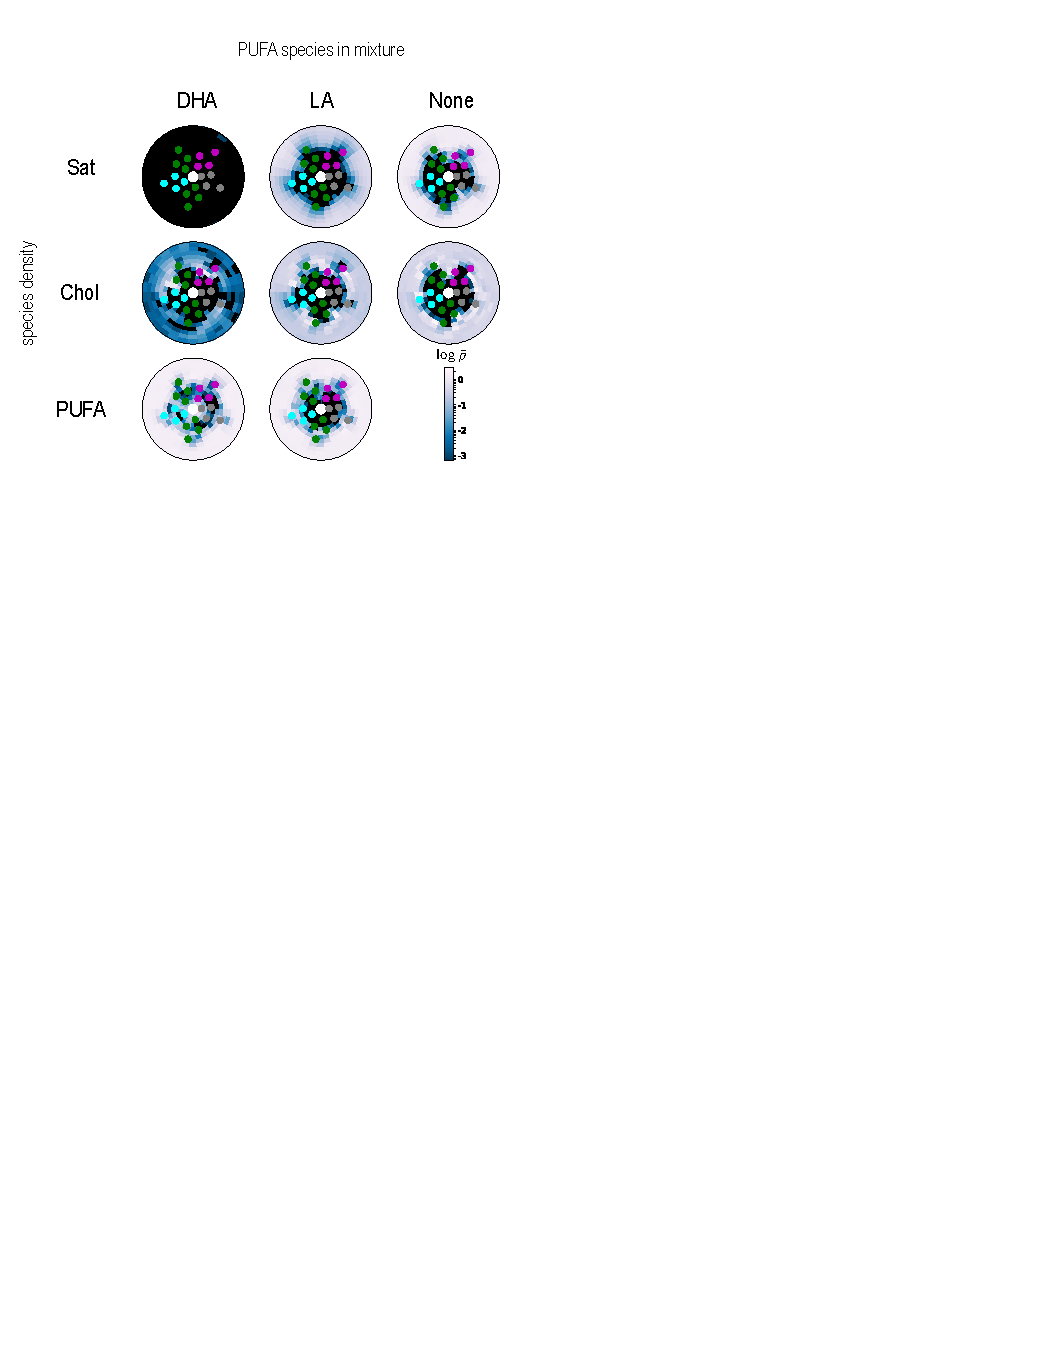
\includegraphics[width=1\linewidth]{Fig3.pdf}
		\caption{Heat maps depicting specific lipid densities averaged over three replicas at DPPC:PUFA:CHOL 40:40:20. The first row show $\rho_{PUFA}$, the second show $\rho_{DPPC}$, and the third row shows $\rho_{Chol}$. } 
		\label{fig:fig3}
	\end{figure}

	%Heat maps in Figure \ref{fig:fig3} \textbf{b} show the average density of cholesterol $(\rho_{Chol})$ within a membrane. $\rho$ is generally defined by equation \ref{eq:R}. In \ref{fig:fig3}b left, the system has a composition DHA-PE:DPPC:Chol 40:40:20. Chol is found in the $l_o$ domain. However, while $\beta$ subunit is partitioned into the $l_d$ phase, there is significant increase in $\rho_{Chol}$ within the $\beta$ subunit. In \ref{fig:fig3} \textbf{b right} DLiPC:DPPC:Chol 40:40:20, $\rho_{Chol}$ is greatest throughout the protein, with largest value within $\delta$ subunit.

	%Figure \ref{fig:fig3} shows the average of three replicas of PUFA:DPPC:Chol 40:40:20, where the PUFA is either DHA-PE or DLiPC. Protein chain locations are also averaged, resulting in a compressed area. Cholesterol is still observed to partition near or within nAChR and in the $l_o$ phase in systems containing DHA. It is highly dispersed within the bulk membrane and embedded with nAChR in systems with DLiPC. Saturated lipids in both series of systems tend to form the bulk membrane, and do not readily interact with nAChR. PUFAs tend form a dense boundary area around nAChR. Chol is observed to embed within or between subunits indiscriminately.

	\begin{figure}[h!]
		\center
		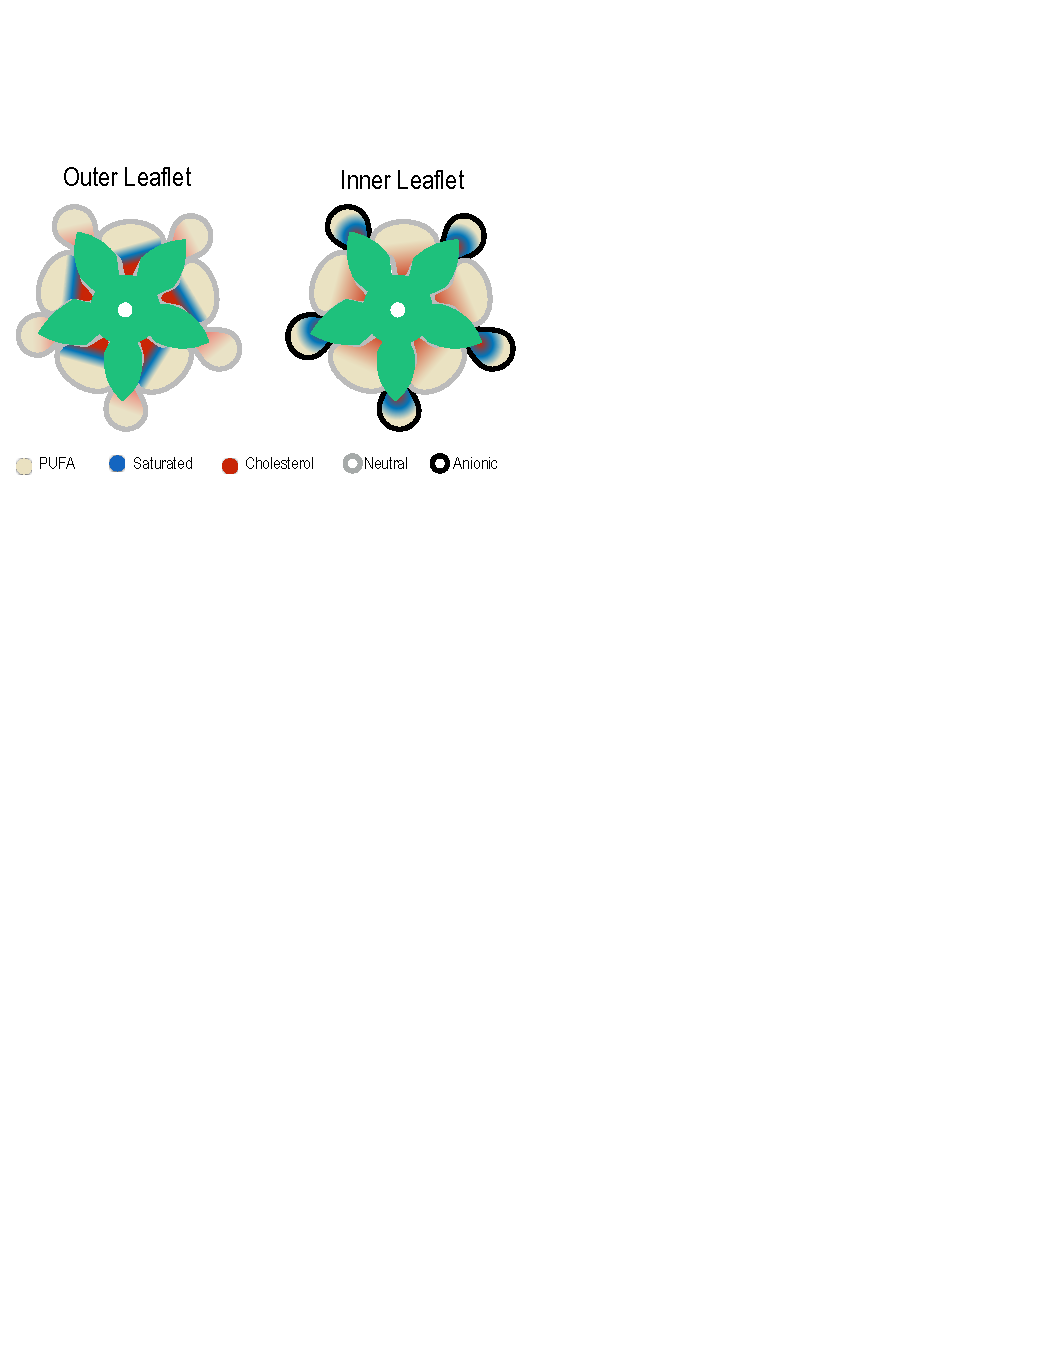
\includegraphics[width=1\linewidth]{Summary.pdf}
		\caption{ Image shows late in trajectory snap-shot. Subimage shows EM density map of the TMD. Blue shows locations of high protein density, white shows low protein density, and red shows an absence of protein.} 
		\label{fig:sum}
	\end{figure}

	 